\documentclass[10pt,twocolumn,a4paper]{article}

% Stile, vincoli formattazione e title block: vedi cim2026.sty
\usepackage{cim2026}

% ================================================================
% NOTA: titolo + autore da finalizzare in fase di submission.
% Versione double-blind: titolo neutro, autore "Anonymous".
\title{Un ambiente python per l’elaborazione granulare:\\
        dal codice alla partitura grafica}

\author{
  \begin{tabular}{c}
    Anonymous\\
    \small [Anonymous]\\
    \small anonymous@anonymous
  \end{tabular}
}
% ================================================================

\begin{document}
\maketitle

%\blfootnote{\small \textit{Copyright: \copyright 2026 Anonymous. This is an open-access article distributed under the terms of the \href{https://creativecommons.org/licenses/by/4.0/}{Creative Commons Attribution License 4.0 International}, which permits unrestricted use, distribution, and reproduction in any medium, provided the original author and source are credited.}}

% ----------------------------------------------------------------
\begin{abstract}
This paper describes a Python environment for deferred-time granular synthesis. 
The system does not synthesise grains from a Gabor primitive but granulates recorded 
material: it belongs to what Lippe terms granular sampling, where the dominant 
expressive parameter is the read position in the source buffer. Granulating at musical 
densities requires specifying thousands of grains per second; the system's problem 
is explicit, legible parametric control over that mass of data. Parameters are specified 
in a declarative approach with a YAML domain-specific language — validated during writing by a 
dedicated Language Server — and interpreted as tendency masks: a central trajectory, 
a deviation range, and an independent per-grain sampling. A decoupled renderer 
architecture supports a per-stream STEMS workflow whose incremental cache and 
DAW-project export keep the edit–listen cycle short enough to inhabit. An 
automatically generated graphical score, whose vertical axis maps the read 
position rather than frequency, closes the feedback loop as a read-only 
diagnostic. We situate the system within the CIM granular tradition and 
discuss what is at stake in choosing deferred time while real time is available.
\end{abstract}

% ================================================================
\section{Introduzione}

Questo lavoro descrive il programma PythonGranularEngine (PGE) per la sintesi granulare in
tempo differito. La sintesi granulare costruisce il suono come
collezione di migliaia di grani, brevi eventi sonori di durata tipica
1-50~ms, e richiede di specificare, direttamente o per via
algoritmica, i parametri di ciascuno. Già la prima implementazione
computer documentata~\cite{Roads1978} osserva che la specifica
esplicita diventa intrattabile non appena la densità supera poche
unità per secondo. Il problema centrale del sistema è quindi il
controllo parametrico: rendere \emph{esplicito} e \emph{leggibile} il
governo di una massa di grani che nessun compositore può razionalizzare
grano per grano.

Una precisazione tassonomica è dovuta fin da subito. \emph{Sintesi
granulare} è qui termine-ombrello per il paradigma; il sistema, nello
specifico, non sintetizza grani da una primitiva di Gabor ma
\emph{granula} materiale registrato: legge e ricompone frammenti di
un campione sorgente. Appartiene cioè al ramo che
Lippe~\cite{Lippe1993cim} distingue come \emph{granular sampling}, la
granulazione di campioni (o micromontage), in cui il parametro
espressivo dominante è la posizione di lettura nel materiale. Questa
collocazione, che riprendo in \S\ref{sec:partitura} e
\S\ref{sec:tradizione}, motiva sia l'asse della partitura sia il
ruolo centrale del \texttt{PointerController}.

Il sistema adotta il tempo differito oggi in una fase storico-informatica in cui il tempo reale 
è tecnicamente disponibile; sulle ragioni di questa scelta
discuto in \S\ref{sec:implicazioni}. L'esposizione muove dal problema
concreto del controllo parametrico e sviluppa tre nuclei principali:
\begin{itemize}
\item optando per un approccio dichiarativo al controllo dei parametri granulari,
  un \emph{domain-specific language}%
  \footnote{Con \emph{domain-specific language} si intende un linguaggio 
  formale progettato per un dominio specifico, in contrapposizione ai 
  linguaggi general-purpose. Non richiede necessariamente una nuova sintassi e
  può appoggiarsi a un formato esistente come \emph{syntax host}, 
arricchendolo di un vocabolario e di una semantica propri del dominio. 
  }
  (DSL), validato da un \emph{Language Server}\footnote{Un \emph{Language Server} è un componente software che analizza 
il testo di un file durante la scrittura e fornisce in tempo reale 
autocompletamento, validazione e documentazione contestuale all'interno 
dell'editor. Il protocollo standard è LSP (\emph{Language Server Protocol}, 
Microsoft 2016).} (orientato alla 
  composizione assistita) durante
  la scrittura e interpretato come \emph{tendency mask} (traiettoria
  centrale, range di deviazione, campionamento per-grano). In particolare
  il nostro DSL sarà qui YAML\footnote{Acronimo ricorsivo di YAML Ain't 
  Markup Language, è un formato di serializzazione dati facilmente 
  leggibile dagli esseri umani.};
\item un sistema che differenzia le voci lungo
  quattro assi ortogonali (\emph{pitch}, \emph{onset}, \emph{pointer}, \emph{pan}) mediante
  strategie intercambiabili (accordo, lineare, stocastico, \dots) e un
  parametro \texttt{scatter} che controlla la variazione di asincronia temporale delle voci;
\item una partitura grafica generata automaticamente, il cui asse
  verticale codifica la posizione di lettura nel buffer sorgente,
  e un workflow di stream audio separati con cache incrementale ed export verso DAW (REAPER),
  che chiude il ciclo di generazione compositiva e verifica.
\end{itemize}
Il paper procede dal basso: prima il sistema (\S\ref{sec:architettura})
e la sua partitura (\S\ref{sec:partitura}), poi il posizionamento
nella tradizione granulare (\S\ref{sec:tradizione}), infine le
implicazioni teorico-compositive (\S\ref{sec:implicazioni}).




% =====================================================================
% §2 — cappello + §2.1 (bozza da integrare in paper.tex)
%
% Labels definiti qui e da usare nelle sottosezioni future:
%   sec:stream-minimo   §2.1  Lo stream minimo
%   sec:griglia         §2.2  La griglia temporale        (ex1_distribution)
%   sec:pointer         §2.3  La posizione di lettura     (ex2_pointer)
%   sec:deviazione      §2.4  Deviazione: ampiezza e probabilità (ex3a/ex3b)
%   sec:voci            §2.5  La molteplicità delle voci  (ex4, ex5)
%   sec:render          §2.6  Dal Grain all'audio
%
% TODO prima della submission:
%   [ ] DOI Zenodo anonimo nella footnote del cappello
%   [ ] valore del residuo RMS nella caption della figura
%   [ ] verificare che i path examples/ex0_identity/... esistano dopo la rinomina
% =====================================================================

% ================================================================
\section{Architettura per l'indagine parametrica}\label{sec:architettura}

Il motore di generazione prevede una fase \emph{dichiarativa}
(la costruzione al momento del parsing di una rappresentazione
intermedia\footnote{Il termine \emph{intermediate representation} (IR) è
mutuato dall'architettura dei compilatori, dove indica la forma che il
codice sorgente assume dopo il parsing e prima della generazione del
codice target: una struttura normalizzata, indipendente dalla sintassi
di input e dal formato di output, su cui operano le trasformazioni.},
nominata da qui in avanti IR) e una \emph{imperativa} (il campionamento
della IR grano per grano in un loop di generazione). La prima realizza
ciò che è già stato anticipato in ambito CIM
da~\cite{DiScipioTisato1993cim}: \emph{«a single rule may instantiate
multiple operations [\dots] a step towards the abstract»}. La seconda
materializza quella dichiarazione in \texttt{Grain}: eventi granulari
immutabili, ciascuno calcolato al proprio tempo $t$.

L'esposizione adotta il metodo del sistema stesso. Si parte dallo
\emph{stream minimo} --- la specifica che si limita a riprodurre il
materiale sorgente --- e si procede per scostamenti, aggiungendo una
deviazione alla volta; ogni listato successivo al primo mostra soltanto
le chiavi aggiunte. Ciascun esempio è una specifica YAML completa ed
eseguibile, accompagnata da una realizzazione (audio e
partitura).\footnote{Specifiche, audio e partiture degli esempi sono
raccolti in un bundle anonimo: DOI Zenodo [TODO]. Dove l'esempio
contiene componenti stocastiche, la specifica determina
l'\emph{andamento} del risultato, non la singola realizzazione
bit-identica; il punto è ripreso in \S\ref{sec:deviazione}.}

% ----------------------------------------------------------------
\subsection{Lo stream minimo: la copia fedele}\label{sec:stream-minimo}

Partiamo dalla dichiarazione di un singolo stream osservando il file
\texttt{ex0\_identity.yml} (Listato~\ref{lst:stream-minimo}).
    \lstinputlisting[
      linerange={3-7},
      language=yaml,
      basicstyle=\ttfamily\fontsize{7.5}{9}\selectfont,
      label=lst:stream-minimo,
      caption={Lo stream minimo: le sole quattro chiavi obbligatorie
      (\texttt{ex0\_identity.yml}).}
    ]{examples/ex0_identity/ex0_identity.yml}

A livello macroscopico la sintassi prevede una lista di stream, ciascuno
un dizionario di chiavi. Le quattro chiavi del listato ---
\texttt{stream\_id}, \texttt{onset}, \texttt{duration}, \texttt{sample}
--- sono le sole obbligatorie: fissano l'identità dello stream e bastano
a generarlo. Ogni altro parametro assume il valore di default, e i
default sono scelti perché lo stream minimo ricostruisca fedelmente il
materiale sorgente: grani di 50~ms con finestra di Hann sovrapposti con
fattore~2,\footnote{Il fattore~2 è la condizione di somma costante
(COLA) della finestra di Hann: l'overlap-add restituisce la forma d'onda
di partenza.} letti in avanti a velocità naturale, senza trasposizione
né deviazione per-grano. La Fig.~\ref{fig:stream-minimo-waveform}
verifica empiricamente questa proprietà confrontando il campione
sorgente con il rendering dello stream minimo.

\begin{figure}[h]
    \includegraphics[width=\linewidth]{examples/ex0_identity/ex0_identity_comparison}\\
    \captionof{figure}{Confronto fra il campione sorgente (originale) e
    la forma d'onda prodotta dal rendering dello stream minimo
    (elaborato); residuo RMS fra le due forme d'onda: $-$[TODO]~dB.}
    \label{fig:stream-minimo-waveform}
\end{figure}

Lo stream minimo fissa così il grado zero del sistema: lo stato di
default è la copia fedele, e ogni chiave aggiunta è uno scostamento da
essa. Da qui in avanti, leggere una specifica significherà leggerne gli
scostamenti. È il percorso delle prossime sottosezioni, una deviazione
alla volta: la griglia temporale di emissione dei grani
(\S\ref{sec:griglia}); la posizione di lettura nel materiale
(\S\ref{sec:pointer}), l'asse che per il granular sampling abbiamo
riconosciuto come dominante; l'ampiezza e la probabilità della
deviazione per-grano %(\S\ref{sec:deviazione});
 la molteplicità e
l'indipendenza delle voci %(\S\ref{sec:voci}). 
Chiude la sezione il
percorso inverso, dal \texttt{Grain} all'audio %(\S\ref{sec:render}).







% =====================================================================
% §2.2 — La griglia temporale (esempio: ex1_distribution)
%
% Pattern: domanda musicale -> diff YAML -> lettura della figura ->
%          meccanismo (unica formula) -> aggancio teorico -> ponte a §2.3
%
% TODO prima della submission:
%   [ ] linerange del listato: allineare alle righe reali di
%       examples/ex1_distribution/ex1_distribution.yml (mostrare il diff:
%       density, grain.duration, pointer, distribution)
%   [ ] verificare nome figura: ex1_distribution_waveform.pdf
%   [ ] \cite{Truax1988}: allineare alla chiave reale in refs.bib
% =====================================================================

% ----------------------------------------------------------------
\subsection{La griglia temporale}\label{sec:griglia}

La copia fedele di \S\ref{sec:stream-minimo} poggia su una griglia che
il listato non mostra: i grani nascono a distanza costante, l'intervallo
fra gli onset (\emph{inter-onset time}, IOT) è il passo che garantisce
la condizione di somma costante. Il primo scostamento tocca proprio
questa griglia: che cosa accade quando il metro di emissione dei grani,
a parità di flusso medio, si dissolve in una distribuzione stocastica?

    \lstinputlisting[
      linerange={24-33}, % TODO: allineare al file reale
      language=yaml,
      basicstyle=\ttfamily\fontsize{7.5}{9}\selectfont,
      label=lst:griglia,
      caption={Le chiavi aggiunte allo stream minimo
      (\texttt{ex1\_distribution.yml}).}
    ]{examples/ex1_distribution/ex1_distribution.yml}

Del Listato~\ref{lst:griglia}, la variabile dell'esempio è una sola:
\texttt{distribution}, scritta qui come envelope --- una lista di punti
$[t, v]$ interpolati linearmente, dove con \texttt{time\_mode:
normalized} il tempo è espresso come frazione della durata dello
stream.\footnote{Ogni parametro del sistema accetta indifferentemente
uno scalare o un envelope; la sintassi compare qui per la prima volta e
vale ovunque.} Le altre chiavi sono di servizio, e le dichiariamo come
tali: densità ridotta e grani brevi mantengono i singoli onset leggibili
come impulsi distinti; la testina di lettura è ferma su un punto del
campione, così che nulla cambi \emph{nel} materiale mentre cambia il suo
tempo di emissione (alla posizione di lettura è dedicata la
\S\ref{sec:pointer}).

La Fig.~\ref{fig:griglia-waveform} mostra l'esito sulla forma d'onda. A
sinistra gli impulsi sono equidistanti: dieci grani al secondo a
intervallo fisso, una pulsazione metrica, meccanica. Procedendo verso
destra la spaziatura si disgrega --- coppie, addensamenti, vuoti ---
mentre il flusso medio resta lo stesso: la trasformazione è puramente
ritmica, dal metro al gocciolio irregolare, senza che timbro o densità
media siano toccati.

\begin{figure}[h]
    \includegraphics[width=\linewidth]{examples/ex1_distribution/ex1_distribution_waveform}\\
    \captionof{figure}{Forma d'onda del rendering di
    \texttt{ex1\_distribution}: treno di impulsi sincrono (sinistra) che
    si dissolve in distribuzione asincrona (destra) a densità media
    costante.}
    \label{fig:griglia-waveform}
\end{figure}

Il meccanismo è l'operativizzazione del modello sincrono/asincrono di
Truax~\cite{Truax1988}. Posto $\overline{\mathrm{IOT}} = 1/\mathit{density}$,
con $\mathit{distribution}=0$ ogni grano nasce a distanza fissa
$\overline{\mathrm{IOT}}$; con $\mathit{distribution}=1$ l'intervallo è
campionato uniformemente in $[0,\,2\,\overline{\mathrm{IOT}}]$, che ne
preserva la media; i valori intermedi interpolano linearmente fra i due
regimi. L'envelope su \texttt{distribution} compone così una transizione
dal metrico allo stocastico senza specificare alcun singolo intervallo:
è la regola che istanzia molte operazioni del cappello di
\S\ref{sec:architettura}, vista all'opera sul primo esempio non
deterministico --- due rendering della stessa specifica differiscono nei
singoli IOT, non nell'andamento.

Abbiamo deformato il tempo di \emph{emissione} dei grani tenendo ferma
la lettura. Ma nella granulazione di campioni i tempi in gioco sono due,
e l'altro --- il tempo con cui si percorre il materiale --- è l'asse su
cui questo sistema costruisce la propria espressività.

% =====================================================================
% §2.3 — La posizione di lettura (esempio: ex2_pointer)
%
% Pattern: domanda musicale -> diff YAML (un solo blocco) ->
%          fallimento della waveform -> PRIMA figura-partitura con
%          legenda minima -> meccanismo -> artefatto del freeze ->
%          ponte a §2.4
%
% TODO prima della submission:
%   [ ] linerange del listato: allineare alle righe reali di
%       examples/ex2_pointer/ex2_pointer.yml (mostrare solo il blocco pointer)
%   [ ] verificare nome figura: ex2_pointer_score.pdf
%   [ ] verificare il punto di congelamento (~1,3 s) dopo la taratura
%       definitiva dell'envelope, e che cada su vocale
%   [ ] \cite{Lippe1993cim}: allineare alla chiave reale in refs.bib
% =====================================================================

% ----------------------------------------------------------------
\subsection{La posizione di lettura}\label{sec:pointer}

Nella granulazione di campioni i tempi in gioco sono due: il tempo del
suono registrato e il tempo con cui lo si percorre. Nello stream minimo
coincidono --- è parte della copia fedele --- e lo scostamento
successivo li separa: che cosa accade quando il tempo di lettura si
stacca dal tempo del materiale?

    \lstinputlisting[
      linerange={40-42}, % TODO: allineare al file reale
      language=yaml,
      basicstyle=\ttfamily\fontsize{7.5}{9}\selectfont,
      label=lst:pointer,
      caption={L'unica chiave aggiunta allo stream minimo
      (\texttt{ex2\_pointer.yml}).}
    ]{examples/ex2_pointer/ex2_pointer.yml}

Il diff è un solo blocco (Listato~\ref{lst:pointer}): un envelope sulla
velocità di lettura. Per i primi quattro decimi di secondo
\texttt{speed\_ratio} vale 1 e lo stream \emph{è} la copia fedele di
\S\ref{sec:stream-minimo}; poi la velocità decresce fino a zero e la
testina si arresta a circa 1,3~s nel campione, su una vocale. All'ascolto
è il gesto granulare per antonomasia: la parola che rallenta e si fa
vocale tenuta, il \emph{time-stretch} che degenera in congelamento.

Ma di questa trasformazione la forma d'onda --- lo strumento di verifica
delle Figg.~\ref{fig:stream-minimo-waveform}
e~\ref{fig:griglia-waveform} --- non dà conto: l'energia resta piena e
continua, perché ciò che è cambiato non è \emph{quanta} energia scorre ma
\emph{quale punto} del materiale la genera. Serve una rappresentazione
che mostri la lettura, ed è la partitura grafica che il sistema genera a
ogni rendering (Fig.~\ref{fig:pointer-score}): in ascissa il tempo del
brano, in ordinata la posizione di lettura nel buffer sorgente, ogni
segmento un grano. La traiettoria dichiarata nello YAML vi appare
letteralmente disegnata: la diagonale della lettura naturale che si piega
fino all'orizzontale del congelamento. Alla notazione, qui ridotta alla
sua legenda minima, è dedicata la \S\ref{sec:partitura}.

\begin{figure}[h]
    \includegraphics[width=\linewidth]{examples/ex2_pointer/ex2_pointer_score}\\
    \captionof{figure}{Partitura grafica del rendering di
    \texttt{ex2\_pointer}: ascisse = tempo del brano, ordinate =
    posizione di lettura nel buffer sorgente (0 = inizio, 1 = fine del
    campione); ogni segmento un grano. La diagonale (lettura a velocità
    naturale) decelera fino all'orizzontale (congelamento).}
    \label{fig:pointer-score}
\end{figure}

Il meccanismo è elementare: la posizione di lettura è l'integrale della
velocità, e \texttt{speed\_ratio} ammette qualunque valore --- 1 è la
lettura naturale, 0 il congelamento, i valori negativi la lettura
retrograda. È su questo asse che la granulazione di campioni colloca il
proprio parametro espressivo dominante~\cite{Lippe1993cim}, e l'esempio
mostra perché: stesso materiale, stessa griglia di emissione, e un tempo
musicale interamente altro. Si noti che la specifica è ancora del tutto
deterministica: due rendering coincidono al campione.

Proprio questo determinismo, però, ha un costo udibile. Nel tratto
congelato i grani sono identici e nascono su una griglia metronomica: il
risultato è periodico, un ronzio meccanico che tradisce il granulatore.
Come si scioglie questa rigidità senza rinunciare alla traiettoria
disegnata?



% =====================================================================
% §2.4 — La deviazione per grano: ampiezza e probabilità
%         (esempi gemelli: ex3a_range, ex3b_dephase)
%
% Pattern: risposta alla domanda di §2.3 -> diff gemelli (la sola
%          posizione dell'envelope) -> lettura della figura doppia ->
%          meccanismo (tendency mask + gate ortogonale) -> quadrato 2x2
%          (envelope puro / Truax / gated / micromodulazione-Vaggione)
%          -> riproducibilità (andamento) -> ponte a §2.5
%
% TODO prima della submission:
%   [ ] linerange dei due listati: allineare alle righe reali di
%       ex3a_range.yml (blocco pointer) e ex3b_dephase.yml (pointer+dephase)
%   [ ] verificare nomi figure: ex3a_range_score.pdf, ex3b_dephase_score.pdf
%   [ ] descrittori percettivi (sfocatura progressiva / crepitio crescente):
%       validare all'ascolto e riformulare sull'evidenza reale
%   [ ] numeri della micromodulazione (±1,5 dB; ±15°; ±5 ms; ±5% buffer):
%       aggiornare se i default_jitter cambiano (issue pitch in corso)
%   [ ] \cite{Truax1988} e \cite{Vaggione2002}: allineare alle chiavi reali
%   [ ] figure*: verificare resa a doppia colonna con cim2026.sty
% =====================================================================

% ----------------------------------------------------------------
\subsection{La deviazione per grano: ampiezza e probabilità}\label{sec:deviazione}

La risposta è la deviazione per grano: attorno alla traiettoria
dichiarata, ogni parametro può ricevere, grano per grano, uno scarto
campionato in modo indipendente. Il sistema fattorizza questa
stocasticità in due dimensioni a loro volta indipendenti ---
\emph{quanto} un grano può deviare, e \emph{con quale probabilità} la
deviazione avviene --- ed entrambe accettano envelope. I due esempi di
questa sottosezione sono gemelli costruiti per isolarle: stessa base
(lettura congelata su una vocale, come al termine di
\S\ref{sec:pointer}), stessa banda massima di deviazione; differiscono
per la sola posizione dell'envelope.

\begin{figure*}[t]
    \begin{minipage}{.48\textwidth}
        \centering
        \includegraphics[width=\linewidth]{examples/ex3a_range/ex3a_range_score}
    \end{minipage}\hfill
    \begin{minipage}{.48\textwidth}
        \centering
        \includegraphics[width=\linewidth]{examples/ex3b_dephase/ex3b_dephase_score}
    \end{minipage}
    \captionof{figure}{Partiture dei due gemelli (assi come in
    Fig.~\ref{fig:pointer-score}). A sinistra (\texttt{ex3a\_range})
    cresce l'ampiezza della deviazione: cuneo a riempimento uniforme. A
    destra (\texttt{ex3b\_dephase}) cresce la probabilità: la linea
    centrale persiste mentre la popolazione deviante si infittisce
    sull'intera banda.}
    \label{fig:gemelli}
\end{figure*}

Nel primo gemello l'envelope sta sull'\emph{ampiezza}
(Listato~\ref{lst:mask-range}): il range di deviazione della posizione
di lettura cresce da zero al 35\% del buffer, e --- in assenza di altre
indicazioni --- la maschera è sempre attiva: ogni grano devia.

    \lstinputlisting[
      linerange={36-42},
      language=yaml,
      basicstyle=\ttfamily\fontsize{7.5}{9}\selectfont,
      label=lst:mask-range,
      caption={Gemello A: l'envelope sull'ampiezza della deviazione
      (\texttt{ex3a\_range.yml}).}
    ]{examples/ex3a_range/ex3a_range.yml}

Nel secondo gemello l'envelope si sposta sulla \emph{probabilità}
(Listato~\ref{lst:mask-dephase}): l'ampiezza resta fissa al massimo del
gemello A, e a crescere da 0 a 100\% è la chiave \texttt{dephase} --- la
frazione di grani a cui la deviazione si applica.

    \lstinputlisting[
      linerange={36-43},
      language=yaml,
      basicstyle=\ttfamily\fontsize{7.5}{9}\selectfont,
      label=lst:mask-dephase,
      caption={Gemello B: ampiezza fissa, envelope sulla probabilità
      (\texttt{ex3b\_dephase.yml}).}
    ]{examples/ex3b_dephase/ex3b_dephase.yml}

La Fig.~\ref{fig:gemelli} affianca le due partiture, e le due morfologie
non potrebbero essere più diverse. A sinistra un cuneo: la banda si
allarga con continuità e i grani la riempiono uniformemente, nessuno
resta sulla linea di partenza perché tutti deviano --- di poco
all'inizio, di molto alla fine. A destra la linea centrale persiste per
l'intera durata, mentre una popolazione crescente la abbandona saltando
da subito sull'intera banda: non un allargamento ma una mistura, grani
fedeli e grani devianti in proporzione componibile nel tempo.
All'ascolto, una sfocatura progressiva della vocale contro un crepitio
che si infittisce attorno a una vocale che resta a fuoco. Stessa base,
stessa banda massima: ampiezza e probabilità della deviazione sono assi
indipendenti del controllo.

Il meccanismo sottostante è la \emph{tendency mask} della tradizione
granulare~\cite{Truax1988}: per ogni parametro una traiettoria centrale
nel tempo, un range di deviazione e un campionamento indipendente per
grano (uniforme, centro~$\pm$~range/2; una distribuzione gaussiana è
selezionabile in alternativa). Il gemello A è questo modello classico
all'opera. Il contributo proprio del sistema è il secondo asse: un gate
probabilistico, anch'esso componibile come envelope, che decide grano
per grano \emph{se} la maschera si applica --- il gemello B, dove la
texture non è una banda che si deforma ma una popolazione che migra.

Il quadro delle combinazioni si lascia ora leggere per intero. Senza
range né dephase, il parametro segue l'envelope puro: è il regime
interamente scritto di \S\ref{sec:pointer}. Range senza dephase: la
maschera sempre attiva di Truax (gemello A). Range con dephase: la
maschera \emph{gated} (gemello B). Resta l'ultimo angolo, il dephase
senza alcun range: il gate apre allora deviazioni implicite di entità
minima definite dal sistema --- circa $\pm$1,5~dB sul volume,
$\pm$15\textdegree~sul pan, $\pm$5~ms sulla durata, $\pm$5\% del buffer
sulla lettura --- una micromodulazione che non disegna alcuna
traiettoria ma decorrela la massa grano per grano, nei termini della
\emph{décorrélation microtemporelle} di Vaggione~\cite{Vaggione2002}. Ed
è la risposta minima alla domanda da cui siamo partiti: da sola, senza
nulla di scritto, scioglie il ronzio del congelamento (esempio audio
\texttt{exA\_micro} nel bundle).

Una parola sulla riproducibilità, qui che la stocasticità è in primo
piano: due rendering della stessa specifica producono grani diversi ma
la stessa morfologia. Ciò che lo YAML determina --- ed è lo YAML che il
bundle spedisce --- è l'andamento; la realizzazione allegata ne è
un'istanza.

Tutto ciò che precede riguarda però ancora una voce sola: un'unica
testina di lettura, un'unica griglia di emissione, una massa di grani
indifferenziata. Lo scostamento successivo moltiplica la voce.



% =====================================================================
% §2.5 — La molteplicità delle voci (esempi: ex4_voices, ex5_scatter)
%
% Pattern: risposta al ponte di §2.4 -> quattro assi ortogonali +
%          strategie (DISCIPLINA: nominarne due, registry una volta) ->
%          ex4 = polo deterministico (bit-identico) -> scatter come
%          accoppiamento temporale -> ex5 -> ponte a §2.6
%
% TODO prima della submission:
%   [ ] ex4_voices.yml: fissare num_voices a 5 costante (l'attuale envelope
%       [[0,5],[.5,1],[1,10]] era sperimentale: per la figura a cinque bande
%       parallele e la lettura piu' pulita serve N fisso) e duration 20
%   [ ] linerange dei listati: allineare ai file reali (ex4: blocco voices;
%       ex5: le sole righe distribution + scatter)
%   [ ] verificare nomi figure: ex4_voices_score.pdf, ex5_scatter_score.pdf
%   [ ] B&W check: la separazione delle bande su Y (pointer linear) deve
%       reggere la stampa in scala di grigi anche senza il colore=pitch
%   [ ] valvola di compressione (se la sezione sfora): fondere le due
%       figure in un doppio pannello o ridurre scatter a sola prosa
% =====================================================================

% ----------------------------------------------------------------
\subsection{La molteplicità delle voci}\label{sec:voci}

Moltiplicare la voce significa dichiarare che lo stream non emette un
grano per volta ma $N$ grani coordinati. Se le $N$ voci fossero
identiche, la moltiplicazione sarebbe un puro guadagno d'energia; la
domanda compositiva è come differenziarle senza doverle scrivere una per
una.

Il blocco \texttt{voices} risponde con quattro assi ortogonali di
differenziazione --- trasposizione, ritardo d'attacco, posizione di
lettura, posizione spaziale --- ciascuno governato da una strategia
intercambiabile (il registro è estensibile); la voce~0 è il riferimento
e non riceve offset, le altre si dispongono rispetto a essa.
L'esempio (Listato~\ref{lst:voci}) ne impiega due: una strategia
d'accordo sulla trasposizione e una lineare su lettura e spazio.

    \lstinputlisting[
      linerange={30-41}, % TODO: allineare al file reale
      language=yaml,
      basicstyle=\ttfamily\fontsize{7.5}{9}\selectfont,
      label=lst:voci,
      caption={Il blocco \texttt{voices}: cinque voci differenziate su
      tre assi (\texttt{ex4\_voices.yml}).}
    ]{examples/ex4_voices/ex4_voices.yml}

Cinque voci ricevono i cinque gradi di un accordo di
nona\footnote{L'accordo è qui specificato in semitoni; il sistema
ammette unità microtonali (cents, EDO arbitrari).} --- nella partitura,
dove il colore codifica la trasposizione, cinque colori distinti ---
cinque teste di lettura equidistanti, che sull'asse~Y della
Fig.~\ref{fig:voci-score} si separano in altrettante bande parallele, e
un ventaglio spaziale di 150\textdegree, udibile ma estraneo agli assi
della partitura. Si noti il regime: dopo due sottosezioni di
stocasticità governata, qui ogni strategia è deterministica e il
rendering è bit-identico fra le esecuzioni --- il sistema non sa solo
disperdere, sa anche scrivere.

\begin{figure}[h]
    \includegraphics[width=\linewidth]{examples/ex4_voices/ex4_voices_score}\\
    \captionof{figure}{Partitura di \texttt{ex4\_voices}: cinque bande
    parallele sull'asse della posizione di lettura, una per voce; il
    colore codifica la trasposizione (i cinque gradi dell'accordo).}
    \label{fig:voci-score}
\end{figure}

Le voci così ottenute condividono però ancora la stessa griglia
temporale: i loro grani nascono insieme, sugli stessi istanti della voce
di riferimento. La moltiplicazione non è ancora indipendenza, e
l'indipendenza ha nel sistema un proprio asse: \texttt{scatter}, il
grado di accoppiamento temporale fra le voci. A 0 tutte le voci
condividono la sequenza di intervalli della voce~0; a 1 ciascuna
calcola la propria; i valori intermedi interpolano. Nell'esempio
(Listato~\ref{lst:scatter}) l'unica variabile è l'envelope su
\texttt{scatter}; la distribuzione temporale è tenuta asincrona e
\emph{costante} --- condizione di servizio dichiarata: scatter agisce
solo se la griglia ha contenuto stocastico da diversificare
(\S\ref{sec:griglia}) --- e la densità è bassa perché i singoli onset
restino leggibili.

    \lstinputlisting[
      linerange={36-38}, % TODO: allineare al file reale (distribution + scatter)
      language=yaml,
      basicstyle=\ttfamily\fontsize{7.5}{9}\selectfont,
      label=lst:scatter,
      caption={Le righe decisive di \texttt{ex5\_scatter.yml}: griglia
      asincrona costante, envelope sul solo \texttt{scatter}.}
    ]{examples/ex5_scatter/ex5_scatter.yml}

Nella Fig.~\ref{fig:scatter-score} l'esito è leggibile sull'allineamento
degli onset: a sinistra, con le griglie agganciate, i grani delle
quattro bande cadono sulle stesse ascisse --- colonne verticali che
attraversano le voci; procedendo verso destra le colonne si sfaldano e
ogni banda segue il proprio cammino temporale. All'ascolto, da un
ensemble che articola insieme a quattro flussi che si sfilano l'uno
dall'altro. Qui il non-determinismo rientra, e con esso la
riproducibilità per andamento: le voci si sganciano a ogni esecuzione,
mai negli stessi istanti.

\begin{figure}[h]
    \includegraphics[width=\linewidth]{examples/ex5_scatter/ex5_scatter_score}\\
    \captionof{figure}{Partitura di \texttt{ex5\_scatter}: gli onset
    delle quattro voci, allineati in colonne a sinistra
    (\texttt{scatter}=0), si disaccoppiano verso destra
    (\texttt{scatter}=1).}
    \label{fig:scatter-score}
\end{figure}

Lo stream, le sue deviazioni e le sue voci sono ora interamente
dichiarati. Resta il percorso inverso: come la dichiarazione diventa
suono --- e come il sistema tiene questo percorso abbastanza corto da
poterlo percorrere molte volte.



















% ================================================================
\section{Architettura per l'indagine parametrica}\label{sec:architettura}


Il motore di generazione prevede una fase \emph{dichiarativa} 
(la costruzione al momento del parsing di una rappresentazione intermedia\footnote{Il termine \emph{intermediate
 representation} (IR) è mutuato dall'architettura dei compilatori, dove indica la 
 forma che il codice sorgente assume dopo il parsing e prima della generazione del 
 codice target: una struttura normalizzata, indipendente dalla sintassi di input e 
 dal formato di output, su cui operano le trasformazioni.}, nominata da qui in avanti IR)
e una \emph{imperativa} (il campionamento
della IR grano per grano in un loop di generazione).
La prima realizza ciò che è già stato anticipato in ambito CIM da~\cite{DiScipioTisato1993cim}: \emph{«a single rule may instantiate multiple
operations [\dots] a step towards the abstract»}.
La seconda materializza quella dichiarazione in \texttt{Grain}: 
eventi granulari immutabili, ciascuno calcolato al proprio tempo $t$.

Le sottosezioni seguenti sviluppano questa struttura: 
dalla specifica YAML alla IR, dal loop di generazione 
al \texttt{Grain} come risultato materializzato.












\subsection{Dal DSL YAML alla IR parametrica}
Partiremo dalla dichiarazione di un singolo stream osservando il file \texttt{ex5\_esempio1.yml} (Listato~\ref{lst:stream-minimo}).
    \lstinputlisting[
      linerange={3-7},
      language=yaml,
      basicstyle=\ttfamily\fontsize{7.5}{9}\selectfont,
      label=lst:stream-minimo,
      caption={Specifica YAML dello stream minimo (\texttt{ex5\_esempio1.yml}).}
    ]{examples/ex0_identity/ex0_identity.yml}

A livello macroscopico la sintassi prevede una lista di stream, ciascuno un 
dizionario di chiavi. 
Le quattro chiavi del listato --- \texttt{stream\_id}, \texttt{onset},
\texttt{duration}, \texttt{sample} --- sono le sole obbligatorie: fissano l'identità
dello stream e bastano a generarlo. Ogni altro parametro assume il
valore di default, e i default sono scelti perché lo stream minimo
ricostruisca fedelmente il materiale sorgente: grani di 50~ms
con finestra di Hann sovrapposti con fattore~2,\footnote{Il fattore~2 è la condizione di somma costante
  (COLA) della finestra di Hann: l'overlap-add restituisce la forma
  d'onda di partenza.} letti in avanti a
velocità naturale, senza trasposizione né deviazione per-grano.
La Fig.~\ref{fig:stream-minimo} verifica
empiricamente questa proprietà confrontando il campione sorgente con
il rendering dello stream minimo. Lo stato di default è dunque la
copia fedele, e ogni chiave aggiunta è uno scostamento da essa.
 

\begin{figure}[h]
    \includegraphics[width=\linewidth]{examples/ex0_identity/ex0_identity_comparison}\\
    \captionof{figure}{Confronto fra il sorgente (originale) e la forma d'onda
    prodotta dal rendering dello stream minimo (elaborato).}\label{fig:stream-minimo}
\end{figure}





È su questa base che opera il front-end del motore. Il parser e il
\texttt{ParameterOrchestrator} leggono le chiavi, le validano e le
abbassano nella IR: ogni dichiarazione --- valore statico, inviluppo,
range di deviazione --- diventa un oggetto \texttt{Parameter}
tipizzato e valutabile nel tempo, normalizzato rispetto alla sintassi
YAML e indipendente dal numero e dalla disposizione concreta dei
grani. In questo stadio i parametri sono oggetti «dormienti»:
contengono la legge del valore, ma non lo hanno ancora emesso per
generare alcun grano. È su questa IR che i controllori opereranno,
interrogandola istante per istante (\S\ref{sec:controllers}); nella
distanza fra la dichiarazione e questo campionamento sta il passaggio
dal dichiarativo all'imperativo annunciato in apertura di
sezione.\footnote{A livello implementativo le chiavi si dividono in
  due famiglie: il \emph{contesto} (identità e regole di processo
  dello stream, dataclass immutabili propagate a tutti i controllori)
  e i \emph{parametri di sintesi}, descritti da oggetti
  che dichiarano dove leggere il valore nello
  YAML, il default, la chiave del range di deviazione e quella del
  gate probabilistico.}



  



Nel regime additivo il \texttt{Parameter} è composto da una traiettoria
centrale $c(t)$ (l'inviluppo), un range di deviazione $s(t)$, anch'esso
scalare o inviluppo, e una strategia di campionamento (uniforme o
gaussiana). Il modello di controllo è la \emph{tendency mask} di
Truax~\cite{Truax1988}: per ogni grano si campiona
$v_n \sim \mathcal{D}(c(t_n),\,s(t_n))$ in modo indipendente dal grano
precedente, senza memoria di stato. Un secondo livello, il
\texttt{ProbabilityGate} associato alla chiave \texttt{dephase}, decide
\emph{se} la deviazione si applichi al grano corrente, secondo una
probabilità costante o time-varying. Gate e range sono ortogonali: il
valore fissa l'intenzione, l'inviluppo la generalizza nel tempo, il gate
sceglie dove la generalizzazione lascia spazio alla casualità i.i.d.\
del singolo grano.

Il programma di un'interfaccia dichiarativa ad alto livello per la
granulazione (\emph{«a single rule may instantiate multiple operations [\dots] a step towards the abstract»}) è enunciato in ambito CIM da
Di~Scipio e Tisato~\cite{DiScipioTisato1993cim}~(p.~165).
Una conseguenza diretta di questo vocabolario dichiarativo è la coppia 
\texttt{density}/\texttt{fill\_factor}: entrambi controllano l'inter-onset time, 
ma con intenzioni diverse. \texttt{density} è in grani/secondo: il parametro giusto 
quando conta la frequenza assoluta degli eventi, indipendentemente dalla durata del 
grano. \texttt{fill\_factor} esprime la saturazione temporale percepita 
(\texttt{density} = \texttt{fill\_factor}/\texttt{grain\_duration}): 
rimane stabile se \texttt{grain\_duration} varia, perché codifica la proporzione 
di tempo coperta dai grani, non il loro conteggio. La differenza tra i due è 
inudibile finché \texttt{grain\_duration} è costante; emerge quando è un inviluppo.







\begin{figure}[h]
  \centering
  \begin{tikzpicture}[
  font=\footnotesize,
  >=Latex,
  box/.style={rounded corners=2pt, draw=black, semithick, align=center, inner sep=3pt},
  yaml/.style={box, minimum width=30mm},
  orch/.style={box, minimum width=30mm},
  par/.style={box, minimum width=30mm, minimum height=6.5mm},
  param/.style = {draw=black, thin, rounded corners=1pt,
                  align=center, inner sep=1pt, fill=white,
                  minimum width=13mm, minimum height=3.5mm,
                  font=\tiny\ttfamily},
  ctrl/.style={box, minimum width=14mm, minimum height=7mm},
  flow/.style={->, semithick, draw=black},
  query/.style={->, semithick, draw=black, dashed},
  zone/.style={rounded corners=4pt, draw=black!45, dashed, inner sep=6pt},
  zlabel/.style={font=\scriptsize\itshape, text=black!45},
  zContr/.style  = {draw=black!35, dashed, rounded corners=3pt,
                  inner sep=2pt, fill=black!4},
]
% ---- YAML ----
\node[yaml] (yaml)
  {\textbf{File \texttt{.yml}}};
% ---- Orchestrator ----
\node[orch, below=4mm of yaml] (orch)
  {\texttt{ParameterOrchestrator}};

% Parameters grid — change \Ncols/\paramdx/\paramdy to reshape
% \Ncols=2: zona ~31mm, lascia ~46mm a destra per il callout
\def\Ncols{2}
\def\paramdx{14}   % horizontal step, mm
\def\paramdy{4.5}  % vertical step, mm
\coordinate (parambase) at ([yshift=-10mm] orch.south);
\foreach \lbl [count=\i from 0] in {
  {dens/fill},{distrib.},{ptr\_start},
  {speed},{loop\_*},{pitch},
  {gr\_duration},{envelope},{volume},
  {pan},{reverse},
  {\ldots}%
}{
  \pgfmathsetmacro{\col}{int(mod(\i,\Ncols))}
  \pgfmathsetmacro{\row}{int(\i/\Ncols)}
  \pgfmathsetmacro{\xoff}{(\col - (\Ncols-1)/2.0)*\paramdx}
  \pgfmathsetmacro{\yoff}{\row*\paramdy}
  \node[param] at ([xshift=\xoff mm, yshift=-\yoff mm] parambase) (param\i) {\lbl};
}


% zone box per la IR
\begin{scope}[on background layer]
  \node[zone, fit=(param0)(param1)(param2)(param3)(param4)(param5)(param6)(param7)(param8)(param9)(param10)(param11)] (zir) {};
\end{scope}
\node[zlabel, above left=0mm and 5mm of zir.north, anchor=south east, align=right]
  {\textbf{IR}};

\draw[flow] (yaml) -- (orch);
\draw[flow] (orch) -- (zir.north);

% ---- Callout: struttura interna di Parameter (zoom da param5, col destra mediana) ----
\node[
  draw=black, thin, rounded corners=2pt,
  right=6mm of zir.east, anchor=west,
  font=\tiny\ttfamily,
  align=left, inner sep=4pt,
  fill=white
] (pzoom) {%
  \begin{tabular}{@{}l@{\ }l@{}}
    \multicolumn{2}{@{}l}{\normalfont\scriptsize \texttt{Parameter}} \\[1pt]
    value:      & float $|$ Envelope \\
    mod\_range: & float $|$ Envelope \\
    distrib.:   & DistrStrategy \\
    prob\_gate: & Gate \\
    bounds:     & ParamBounds \\
  \end{tabular}%
};
% Linee zoom divergenti da param5 (pitch, col destra mediana) verso callout
\draw[dashed, black!35, thin] (param5.north east) -- (pzoom.north west);
\draw[dashed, black!35, thin] (param5.south east) -- (pzoom.south west);

\end{tikzpicture}

\caption{pino}
\end{figure}









\subsection{Dal grano allo stream}
L'unità atomica è il \texttt{Grain}: una dataclass immutabile descritta da otto campi:
onset, durata, posizione di lettura nel sample, rapporto di
trasposizione, volume, pan, e due indici di tabella (sample e
finestra). La sua unica responsabilità è descriversi. Mantenerlo come
oggetto anche dopo la generazione è la scelta
che definisce l'approccio in tempo differito:
a differenza di ambienti real-time chiusi, dove il grano è
calcolato dentro il grafo DSP e svanisce nel segnale, qui l'output
della generazione resta un corpus ispezionabile.

\lstinputlisting[language=Python,
  linerange={3-4,9-16},
  label=lst:grain,
  caption={La dataclass \texttt{Grain}: otto campi, immutabile (\texttt{frozen}) e con \texttt{slots} per contenere il costo in memoria su grandi quantità di istanze.}]
  {../raw/PythonGranularEngine/src/core/grain.py}

Il livello immediatamente superiore è la classe \texttt{Stream}: dato uno
spazio di parametri e una densità, esso \emph{genera} la lista ordinata
di istanze di \texttt{Grain} che lo realizzano. Questo
passaggio dal singolo grano alla sua organizzazione di livello
superiore è il pattern di base della granulazione algoritmica fin da
~\cite{Roads1978}, dove il front-end calcola da una specifica compatta la \emph{nota-list}
completa per il motore di sintesi.


Tra stream e grano si colloca la \emph{voce}. 
Essa rappresenta un
insieme di \emph{offsets} (su \emph{pitch}, \emph{onset}, \emph{pointer} e \emph{pan}) che il
\texttt{VoiceManager} calcola e fonde in ciascun grano al
momento della generazione (\S\ref{sec:multivoce}).
Da un punto di vista mereologico lo stream 
è composto di grani, mentre la voce è un modo di partizionare questi ultimi all'interno
di uno stream. 
Per questo in \texttt{Stream} le voci sono 
\texttt{List[List[Grain]]} ma non vengono mai reificate allo come classi. Questa struttura conserva l'appartenenza 
di ogni grano alla sua voce nella prospettiva della generazione della partitura grafica 
che la leggerà nelle n bande parallele(\S\ref{sec:partitura}). L'architettura
così descritta è visibile nella \emph{pipeline}(Fig.~\ref{fig:arch}).

\begin{figure}[t]
  \centering
  \begin{tikzpicture}[
      node distance=4pt and 4pt,
      every node/.style={font=\fontsize{7}{8}\selectfont},
      box/.style={draw, rectangle, minimum height=4mm, inner sep=2pt,
                  align=center, font=\fontsize{7}{8}\ttfamily},
      lbl/.style={align=center, font=\fontsize{7}{8}\ttfamily},
      arr/.style={-{Latex[length=1.4mm]}, thick}
    ]
\node[box] (yaml) {YAML};
\node[box, right=10pt of yaml] (gen) {Generator};
\node[box, below=10pt of gen] (ir)
      {Stream / VoiceManager / Controller$\times$4};
\node[lbl, below=5pt of ir] (irlbl)
      {List[List[Grain]]};
\node[box, below=5pt of irlbl] (renderer)
      {AudioRenderer (ABC)};
\node[box, below=5pt of renderer] (np)
      {Numpy\\AudioRenderer};
\node[lbl, below=5pt of np] (aif1) {.aif};
\node[box, right=5pt of renderer, align=center] (cache)
      {Stream\\CacheManager\\\fontsize{6}{7}\selectfont SHA-256\\\fontsize{6}{7}\selectfont (STEMS)};
\node[box, left= 5pt of renderer, align=center] (rp)
      {ReaperProject\\Writer};
\node[lbl, below=10pt of rp] (rpp) {.rpp};
\draw[arr] (yaml) -- (gen);
\draw[arr] (gen)  -- (ir);
\draw[arr] (ir)   -- (irlbl);
\draw[arr] (irlbl)-- (renderer);
\draw[arr] (renderer) -- (np);
\draw[arr] (np) -- (aif1);
%\draw[arr] (ir) to[bend right=15] (rp.north);
\draw[arr, dashed] (ir) to (rp.north);
\draw[arr, dashed] (rp) -- (rpp);
\draw[arr, dashed] (aif1.west) to[bend left=25] (rp.south east);
\draw[arr, dashed] (cache) to[bend left=15] (np);
\end{tikzpicture}

\caption{Pipeline del motore di elaborazione. Il \texttt{Generator} legge lo YAML e
  costruisce gli \texttt{Stream}; ogni stream genera la propria
  \texttt{List[List[Grain]]} (i grani indicizzati per voce). Il rendering
  (disaccoppiato dietro l'astrazione \texttt{AudioRenderer}) in figura è
  basato sulla libreria Python NumPy, ma la stessa interfaccia ospita back-end
  alternativi (es.\ Csound). Le frecce continue sono la catena di
  trasformazione (YAML\,$\to$\,grani\,$\to$\,audio); quelle tratteggiate
  sono relazioni ausiliarie, esterne ad essa: lo \texttt{StreamCacheManager},
  che con un fingerprint SHA-256 per-stream evita di ricompilare gli
  stream invariati, e il \texttt{ReaperProjectWriter} che riporta
  la struttura temporale degli stream in un progetto DAW referenziando i \texttt{.aif} prodotti dall'export.}\label{fig:arch}
\end{figure}















\subsection{Inviluppi e cicli}\label{sec:inviluppi}

L'inviluppo è il meccanismo che trasforma un parametro da costante a
funzione del tempo $f(t)\to v$, definita a tratti su breakpoint con
interpolazione lineare, cubica (tangenti Fritsch-Carlson, monotona e
senza overshoot) o a gradino. Oltre ai breakpoint espliciti, un
\emph{formato compatto} genera $N$ ripetizioni di un pattern espresso in
percentuale del ciclo, la cui durata può essere distribuita in modo
uniforme, esponenziale (\emph{accelerando}), logaritmico
(\emph{ritardando}) o geometrico:

\begin{lstlisting}[language=yaml, basicstyle=\ttfamily\fontsize{7.5}{9}\selectfont]
# macro: una rampa di volume su 30 s
volume:  [[0, -12], [30, 0]]

# micro: densita' 5->50 per ciclo, 8 cicli in accelerando
density: [[[0, 5], [100, 50]], 30, 8, 'linear', 'exponential']
\end{lstlisting}
Lo stesso oggetto descrive una rampa lenta di volume su trenta secondi o
un pattern ritmico-granulare di densità ripetuto in accelerando: la
distanza fra automazione macro-formale e modulazione micro-temporale,
nel DSL, è solo questione di scala dei breakpoint. La forma normalizzata
(coordinate temporali in $[0,1]$ scalate sulla durata dello stream)
disaccoppia il disegno dell'inviluppo dalla durata effettiva: una
sezione resta riusabile a durate diverse.

L'inviluppo è dunque l'ossatura della variazione temporale del
sistema --- ma quanto in profondità penetri dipende dalla natura del
parametro, ed è qui che si legge il confine dell'astrazione. Per i
parametri continui l'inviluppo è sia la traiettoria centrale $c(t)$ sia
l'ampiezza della deviazione $s(t)$: la \emph{tendency mask} di Truax
nella sua forma piena, una maschera i cui bordi si muovono nel tempo.
Per la finestra del grano, categorica, sopravvive solo come la
\texttt{curve} che pilota una transizione probabilistica fra forme
discrete. Per \texttt{reverse}, binario, sparisce dal valore: lo stato
di base insegue il segno della velocità del pointer --- a sua volta un
inviluppo --- mentre una probabilità per-grano decide il flip. Un solo
idioma attraversa così il continuo, il categorico e il binario, e
raggiunge ciascun asse fin dove il suo dominio lo consente.


\subsection{Controllori e generazione dei grani}\label{sec:controllers}

La IR parametrica è interrogata da quattro controllori ortogonali,
ciascuno responsabile di un asse del grano. Il \texttt{DensityController}
traduce densità (o fill factor) in una sequenza di inter-onset time, la
cui distribuzione segue il modello di Truax~\cite{Truax1988} fra \emph{sincrono}
(metronomo perfetto, \texttt{distribution}~$=0$) e \emph{asincrono}
(campionamento uniforme su $[0,\,2\cdot\text{IOT}]$,
\texttt{distribution}~$=1$), con blend lineare governato da un
inviluppo. La differenza è udibile e visibile: a \texttt{distribution}~$=0$
i grani escono a intervalli regolari --- un treno pulsato, metronomico;
a \texttt{distribution}~$=1$ gli onset si disperdono in un tappeto
diffuso, senza periodicità percepibile. La Fig.~\ref{fig:distribution}
rende il passaggio leggibile sulla forma d'onda dell'esempio
\texttt{ex2\_distribution}, dove \texttt{distribution} sale da $0$ a $1$:
gli impulsi regolari di sinistra si sfrangiano nel disordine di destra.
Il \texttt{PointerController} determina la posizione di lettura nel
sample: velocità di scansione (anche negativa, lettura all'indietro),
finestra di loop statica o mobile nel tempo, deviazione per-grano. Il
\texttt{PitchController} applica la trasposizione attraverso un'unità di
misura selezionabile --- semitoni, cents, divisioni arbitrarie
dell'ottava (\textsc{edo}) o ratio diretto --- ricondotta a un fattore di
frequenza da un'unica interfaccia di conversione; il
\texttt{WindowController} seleziona la finestra del grano
da un registro pre-inizializzato alla creazione dello stream (hanning,
gaussian, le asimmetriche expodec/exporise di tradizione Roads), con
transizioni probabilistiche o multi-stato fra finestre.

È nello \texttt{Stream} che i quattro assi si compongono in eventi. La
generazione è un cammino nel tempo: un cursore parte dall'inizio dello
stream e avanza di un inter-onset time alla volta; a ogni passo i
controllori, interrogati al tempo corrente, emettono un \texttt{Grain}
immutabile.

\begin{lstlisting}[language=Python,basicstyle=\ttfamily\fontsize{7.5}{9}\selectfont]
def generate_grains(self):
    grains = []
    t = 0.0
    while t < self.duration:
        dur = self.grain_duration.get_value(t)            
        grains.append(self._create_grain(t, dur))         
        t += self._density.calculate_inter_onset(t, dur)  
    return grains
\end{lstlisting}

Tre cose si leggono in queste poche righe. Il cursore non avanza di un
passo fisso: l'incremento è l'IOT calcolato dal \texttt{DensityController}
\emph{al tempo corrente}, ed è qui che la griglia sincrono/asincrona
appena descritta prende forma istante per istante. Ogni grano campiona
poi i propri parametri al proprio $t$: è il punto in cui gli inviluppi
entrano nella generazione e in cui, per i parametri continui, agisce il
campionamento \emph{tendency mask} già descritto (\S\ref{sec:inviluppi}).
Infine, l'uscita non è un segnale ma una lista ordinata di grani:
il corpus reificato è interrogabile prima ancora di essere reso in
audio.

Il listato mostra la logica a voce singola. Il sistema reale avvolge
questo cammino in $N$ cursori temporali paralleli, uno per voce, che
possono divergere nel tempo: è il tema della \S\ref{sec:multivoce}. Ma
la struttura temporale di base --- cursore, IOT variabile, campionamento
per-grano --- è questa, e la lista che ne risulta è ciò che la partitura
grafica rilegge come bande sull'asse tempo\,$\times$\,posizione
(\S\ref{sec:partitura}).

\begin{figure}[t]
  \centering
  \includegraphics[width=\columnwidth]{examples/ex1_distribution/ex1_distribution_waveform.pdf}
  \caption{Forma d'onda dell'esempio \texttt{ex2\_distribution} (20~s):
    \texttt{distribution} sale da $0$ (sincrono) a $1$ (asincrono).
    Gli impulsi regolari e periodici di sinistra si disperdono
    progressivamente nel tappeto irregolare di destra. La densità è
    bassa per rendere visibili i singoli onset.}\label{fig:distribution}
\end{figure}

\subsection{Multi-voce dichiarativo}\label{sec:multivoce}

La granulazione produce polifonia da decenni. Truax distribuiva fino a
quindici voci sul DMX-1000, e ogni granulatore in tempo reale, da
EmissionControl2~\cite{Roads2021} ai sistemi modulari e commerciali,
sovrappone più stream simultanei. In questi sistemi il criterio con cui
le voci si differenziano è fissato a priori: una dispersione
stocastica, una modulazione a inviluppo applicata in modo uniforme a
ogni parametro (in EC2 una matrice di sei LFO con deviazione casuale
per-grano~\cite{Roads2021}), oppure un singolo schema di trasposizione
come lo \emph{harmonization scheme} a fondamentale $F=4$ di
Truax~\cite{Truax1994}. Il compositore regola l'ampiezza della
differenziazione, non il metodo che la produce.

Qui le voci sono trattate altrimenti. Uno stream è distribuito in $N$
voci differenziate lungo quattro assi ortogonali (pitch, onset,
pointer, pan); su ciascun asse il criterio di differenziazione è una
strategia intercambiabile, selezionata da una singola chiave
dichiarativa (Tab.~\ref{tab:voci}). La voce~0 è il riferimento e non
riceve offset.


\begin{lstlisting}[language=yaml, basicstyle=\ttfamily\fontsize{7.5}{9}\selectfont]
voices:
  num_voices: 4
  pitch:        {strategy: chord,  chord: maj7}
  onset_offset: {strategy: linear, step: 0.05}
  pan:          {strategy: linear, spread: 90}
\end{lstlisting}

\begin{table}[t]
  \centering\small
  \begin{tabular}{@{}ll@{}}
    \hline
    \textbf{Asse} & \textbf{Strategie}\\
    \hline
    pitch   & step, range, chord, stochastic, spectral\\
    onset   & linear, geometric, stochastic\\
    pointer & linear, stochastic\\
    pan     & linear, additive, random\\
    \hline
  \end{tabular}
  \caption{Assi di differenziazione multi-voce e relative strategie.
    Ogni strategia accetta parametri scalari o inviluppo.}\label{tab:voci}
\end{table}

Le strategie sono oggetti registrati in un registro per asse, non
un insieme chiuso di modalità predefinite, e seguono lo stesso schema
\emph{Strategy}/\emph{Factory} che organizza il layer di rendering
(\S\ref{sec:renderer}). Una nuova strategia di voce, un diverso schema
di pitch o una diversa distribuzione del pointer, si aggiunge come
sottoclasse registrata a runtime, senza toccare il nucleo del sistema.
La differenziazione polifonica è perciò aperta all'estensione nel senso
dell'Open-Closed Principle, come il layer di rendering: là si
aggiungono back-end, qui si amplia il vocabolario della polifonia. Le
strategie disponibili di serie contano meno di questa proprietà:
trattare la differenziazione di voce come uno spazio di algoritmi
estensibile è ciò che distingue l'approccio da un quadro di parametri
prefissato.

Due proprietà discendono dall'integrazione con il resto del DSL. Poiché
ogni parametro scalare di strategia accetta un inviluppo, e
\texttt{num\_voices} è a sua volta una funzione del tempo, la polifonia
varia nella forma e nel numero: un cluster monofonico può aprirsi in un
accordo, uno spread di pan allargarsi, le voci attivarsi e spegnersi nel
corso dello stream. Ciascun asse si compone inoltre su tre livelli
distinti --- la traiettoria di base del controllore, l'offset di voce e
la deviazione per-grano --- così che il valore finale del grano è
$\text{base}(t) + \text{offset}_{\text{voce}} + \text{jitter}(t)$:
controllo macro-formale, differenziazione di voce e singolarità del
grano operano sullo stesso asse senza confondersi.

Resta un asse di differenziazione che non agisce sul valore del grano ma
sul suo \emph{tempo}. La generazione avanza, per ciascuna voce, lungo un
cursore temporale indipendente, e il parametro \texttt{scatter} decide
come questi cursori procedano l'uno rispetto all'altro. A
\texttt{scatter}~$=0$ tutte le voci condividono l'inter-onset time della
voce di riferimento: le griglie ritmiche restano agganciate e la
differenziazione è solo di valore. A \texttt{scatter}~$=1$ ciascuna voce
calcola il proprio IOT in modo indipendente e le griglie slittano l'una
sull'altra; i valori intermedi ne sono un blend lineare (Fig.~\ref{fig:scatter}). È, in sostanza,
la distribuzione sincrono/asincrono di Truax portata dal singolo stream
alla relazione fra le voci: là decideva la regolarità della griglia di una
voce, qui decide quanto le griglie di voci diverse restino solidali.
Diversamente dall'\texttt{onset}, che sfasa la griglia di una quantità
fissa per voce, \texttt{scatter} stabilisce se le griglie restino rigide
insieme o divergano; e poiché accetta un inviluppo, le voci possono
agganciarsi e sganciarsi nel corso dello stream --- da un unisono ritmico
a uno sciame di camminate temporali distinte.

\begin{figure}[t]
  \centering
  \includegraphics[width=\columnwidth]{examples/ex5_scatter/ex5_scatter_score.pdf}
  \caption{Partitura dell'esempio \texttt{ex4\_scatter} (20~s): quattro
    voci su quattro bande di lettura distinte (\texttt{pointer} lineare),
    ciascuna di un colore (accordo \texttt{maj7}); \texttt{scatter} sale
    da $0$ a $1$ mentre \texttt{distribution} resta asincrono e costante.
    A sinistra le voci condividono lo stesso inter-onset time e gli onset
    cadono in colonne allineate fra le bande; a destra ciascuna voce
    segue il proprio cammino temporale e l'allineamento si dissolve. La
    densità è bassa per rendere visibili i singoli onset.}\label{fig:scatter}
\end{figure}

Nessuno dei singoli elementi è nuovo, e va riconosciuto. I quattro assi
sono il corredo parametrico consueto della granulazione; la dispersione
stocastica risale a Truax; la decorrelazione spaziale per voce è in
Vaggione~\cite{Vaggione2002}. Sul piano del metodo il precedente più
vicino è CMask~\cite{Bartetzki1997}, che per ogni parametro lascia
scegliere fra generatori diversi (costante, tendency mask,
distribuzioni, random walk); resta però un vocabolario chiuso, interno
a un linguaggio di scripting batch, ampliabile solo modificandone il
codice. La combinazione qui proposta, differenziazione per-asse
selezionata in modo dichiarativo e insieme aperta all'estensione a
runtime nella granulazione di campioni, non risulta documentata altrove
nella letteratura esaminata.

All'ascolto le strategie deterministiche e quelle stocastiche divergono
nettamente: una \texttt{pitch:chord} produce un impasto armonico
stabile, dove le voci si fondono in un timbro composito; una
\texttt{pitch:stochastic} disperde le voci in un pulviscolo
microtonale. La Fig.~\ref{fig:voices} mostra l'esempio
\texttt{ex3\_voices}: un accordo di dominante nona (\texttt{dom9}) su
voci distribuite linearmente nel pan e in altrettante posizioni di
lettura, con un numero di voci che varia nel tempo --- \texttt{num\_voices}
è un inviluppo che parte da cinque, si contrae a una sola voce a metà
dello stream e si riapre a dieci alla fine. La polifonia è perciò una
figura nel tempo, non un dato fisso: il cluster si chiude in un'unica
banda e poi si riapre, e quando le voci eccedono le cinque note
dell'accordo i gradi si ripetono all'ottava superiore. In partitura ogni
voce attiva appare come una banda parallela --- una per posizione di
lettura --- colorata in base al \texttt{pitch\_ratio} che l'accordo le
assegna; il numero di bande segue l'inviluppo di \texttt{num\_voices}, e
rende visibile la contrazione e la successiva apertura. Poiché qui
nessuna strategia è stocastica, l'esempio è bit-identico a ogni
esecuzione: due rendering producono lo stesso output campione per
campione.

\begin{figure}[t]
  \centering
  \includegraphics[width=\columnwidth]{examples/ex4_voices/ex4_voices_score.pdf}
\caption{Partitura dell'esempio \texttt{ex3\_voices} (20~s): accordo
    \texttt{dom9}, pan e posizioni di lettura distribuiti linearmente,
    con \texttt{num\_voices} che varia nel tempo da cinque a una e poi a
    dieci. Il numero di bande parallele segue l'inviluppo del numero di
    voci.}\label{fig:voices}
\end{figure}

\subsection{Renderer disaccoppiati, cache, export}\label{sec:renderer}

Il layer di rendering è disaccoppiato dietro l'astrazione
\texttt{AudioRenderer}, secondo l'Open-Closed Principle: l'interfaccia
espone due soli metodi atomici --- rendering di un singolo stream e di
stream uniti --- mentre una strategia \texttt{RenderMode} ortogonale
decide il partizionamento dell'output (STEMS, un file per stream; MIX,
un file unico). Aggiungere un back-end è così additivo, una sottoclasse
senza modifiche al nucleo. Il renderer nativo, \texttt{NumpyAudioRenderer},
lavora in memoria senza dipendenze esterne; a titolo di esempio se ne
affianca uno alternativo, \texttt{CsoundRenderer}, che invoca
\texttt{csound} come sotto-processo su uno score testuale, per chi opera
nella tradizione Roads/Csound. La stessa specifica YAML è servita da ogni
back-end senza modifica~\cite{Markidis2024cim}.

Su questa astrazione poggia il workflow che sostiene il loop lungo. In
modalità STEMS ogni stream è renderizzato in un file separato e
\texttt{StreamCacheManager} gli associa un fingerprint SHA-256 del dict
YAML serializzato (con \texttt{sort\_keys}, così l'ordine delle chiavi è
irrilevante); uno stream è \emph{dirty} --- e solo allora ri-renderizzato
--- se il fingerprint cambia, se è nuovo, o se il suo file audio manca.
Gli stream rimossi o rinominati sono ripuliti per garbage collection del
manifest. La posta in gioco è il tempo: su un brano con decine di stream,
soprattutto con un back-end esterno come Csound, una build completa è
dell'ordine dei minuti, e senza cache ogni ritocco a un singolo parametro
la pagherebbe per intero. È la cache a rendere il ciclo \emph{modifica-un-parametro
$\to$ riascolta} abbastanza breve da poter essere abitato: non
un'ottimizzazione, ma la condizione perché il loop lungo non collassi
sotto i propri tempi di render.

Due meccanismi chiudono il workflow verso l'ascolto e il montaggio. Una
logica di solo/mute per stream, dichiarata nello YAML, isola un singolo
strato senza toccare la struttura del file. L'export verso DAW chiude poi
il ciclo: \texttt{ReaperProjectWriter} non renderizza audio, ma costruisce
un progetto Reaper che referenzia gli \texttt{.aif} già prodotti,
riportandone la struttura temporale --- onset e durata di ogni stream ---
in timeline senza ricostruzione manuale. L'architettura assume così come
pratica primaria quell'assemblaggio differito che Roads descrive in
Pro~Tools, dove \emph{«detached from real-time constraints, ideas can be
tested, edited, submixed, or deleted at will»}~\cite{Roads2012}, p.~8.

\subsection{Language Server come scaffolding del loop}

Lo schema semantico dei parametri --- nomi, tipi, range, gruppi
mutuamente esclusivi, valori ammessi --- è esposto come JSON Schema e
servito da un Language Server dedicato (\emph{[anonymous]-ls}),
implementato sopra il Language Server Protocol e utilizzabile da
qualunque client conforme. Mentre il compositore scrive il YAML, il
server valida inline contro questo schema (segnalando per esempio i
riferimenti a sample inesistenti) e offre documentazione al passaggio
sulle chiavi e completamento contestuale sui valori. La scrittura della
specifica precede il rendering ed è il punto in cui conviene
intercettare l'errore: senza questo controllo ogni errore emerge solo a
rendering tentato e ogni iterazione del loop si allunga. Con il Language
Server il YAML diventa un'interfaccia di scrittura compositiva che dà
riscontro a ogni modifica.

% ================================================================

\section{La partitura grafica come retroazione}\label{sec:partitura}

La partitura grafica è generata automaticamente dalla stessa IR che
alimenta il rendering. Il compositore non la disegna come input: è il
sistema a produrla come output ispezionabile delle decisioni già
prese. Il suo asse orizzontale è il tempo; il verticale codifica la
\emph{posizione di lettura nel buffer sorgente}. Le rappresentazioni
storiche del controllo granulare hanno usato il verticale per grandezze
diverse --- la frequenza come metafora geometrica (Roads), il valore di
un parametro entro la mask (Truax), una mappa spaziale (GeoGraphy), una
curva di offset come controllo in input (Vocem) --- ma, per quanto ci
risulta nella letteratura qui esaminata, non la posizione di lettura
come \emph{output} misurato del rendering (Tab.~\ref{tab:repr}). Ogni grano è un segno collocato sul piano
tempo~$\times$~posizione-nel-sample; la finestra di loop, la
deviazione del pointer e gli inviluppi dei parametri sono leggibili
come strati sovrapposti (Fig.~\ref{fig:score}). Il singolo grano è reso come
una freccia la cui estensione orizzontale è la sua durata, la cui
posizione verticale è l'offset di lettura nel buffer e il cui verso
codifica la direzione di lettura --- in avanti o, sotto \texttt{reverse},
invertita; la finestra di loop attiva appare come banda, e un pannello allineato sullo stesso asse
temporale traccia gli inviluppi dei parametri continui (densità, volume,
pan). La densità visiva dei segni rende immediatamente percepibile la
stratificazione delle voci e l'addensarsi o il diradarsi del flusso
granulare, informazione che l'ascolto da solo coglie con difficoltà.

La Fig.~\ref{fig:score} è un caso minimo costruito per leggersi a colpo
d'occhio. Un solo stream legge il campione sorgente con una traiettoria
di lettura lenta e continua; l'unico parametro che varia è
\texttt{dephase}, la probabilità che a ciascun grano si applichino le
deviazioni per-grano: la dispersione della posizione di lettura,
l'apertura del pan, un jitter di volume e di durata, e l'inversione del
verso (\texttt{reverse}). A inizio brano la probabilità è
nulla: tutti i grani leggono la posizione prescritta dalla traiettoria
centrale e si allineano in una banda netta, una diagonale sottile che
sale col procedere della testina nel campione. Verso destra la
probabilità cresce fino a $100\%$ e la banda si sfrangia in una nuvola
che si allarga: ogni grano riceve un offset di lettura indipendente, e
la dispersione verticale dei segni \emph{è} la varianza
dell'\texttt{offset\_range} resa visibile. All'ascolto corrisponde il
passaggio da una lettura coerente del campione a una texture diffusa in
cui l'identità della sorgente si sospende. La partitura localizza il
punto esatto in cui ciò accade --- la coordinata temporale dove la linea
diventa nuvola --- che l'orecchio coglie solo come transizione graduale.
Il colore, mappato su \texttt{pitch\_ratio}, resta uniforme: questo
esempio non tocca il pitch. A spostarsi insieme alla nuvola è il verso
di lettura --- frecce che si capovolgono man mano che \texttt{reverse}
entra in gioco con probabilità crescente, rendendo leggibile anche
l'alternarsi fra lettura in avanti e all'indietro.

La partitura chiude il riscontro fra ciò che il YAML dichiara e ciò 
che il rendering produce, rendendo visibile uno scarto che l'ascolto
da solo localizza con fatica. Rispetto ai precursori visivi del
controllo granulare due tratti la distinguono, entrambi leggibili
in Tab.~\ref{tab:repr}: l'asse verticale codifica la posizione di
lettura --- dove l'overlay ASCII delle tendency mask di
Truax~\cite{Truax1988} (Fig.~4), il \emph{polygon} di
AGS~\cite{Roads1978,Roads1988} e la mappa di
GeoGraphy~\cite{ValleLombardo2003} mettevano frequenza o spazio --- e
l'informazione scorre nel verso opposto, dall'output verso il
compositore anziché dal compositore verso la sintesi. L'unico
precedente che adotta lo stesso asse è l'interfaccia del parametro
\emph{offset} di Vocem~\cite{Lopez1998}, ambiente granulare in tempo
reale: tempo sull'orizzontale, posizione nel campione sul verticale.
Là, però, quell'asse ospita una \emph{singola curva di controllo
disegnata in input} --- un inviluppo tracciato per pilotare la lettura
--- non i grani prodotti: niente popolazione granulare, niente
deviazione per-grano, nessun ancoraggio alla forma d'onda sorgente. La
rappresentazione qui descritta inverte il flusso, dall'input di una
traiettoria ideale all'\emph{output} diagnostico dell'intera nuvola di
grani realizzati.

\begin{table}[t]
  \centering\small
  \begin{tabular}{@{}lll@{}}
    \hline
    \textbf{Sistema} & \textbf{Asse Y} & \textbf{Flusso}\\
    \hline
    Truax 1988 (Fig.~4)        & parametro/mask   & input\\
    Roads 1978/88 (polygon)    & frequenza        & metafora\\
    GeoGraphy 2003             & mappa spaziale   & input\\
    Vocem 1998 (offset)        & posizione-buffer & input (1 curva)\\
    questo sistema             & posizione-buffer & output\\
    \hline
  \end{tabular}
  \caption{Rappresentazioni visive nel controllo granulare. Il sistema
    descritto si distingue per asse verticale (posizione di lettura) e
    per direzione del flusso (la partitura è output del rendering, non
    input di controllo).}\label{tab:repr}
\end{table}

\begin{figure}[t]
  \centering
  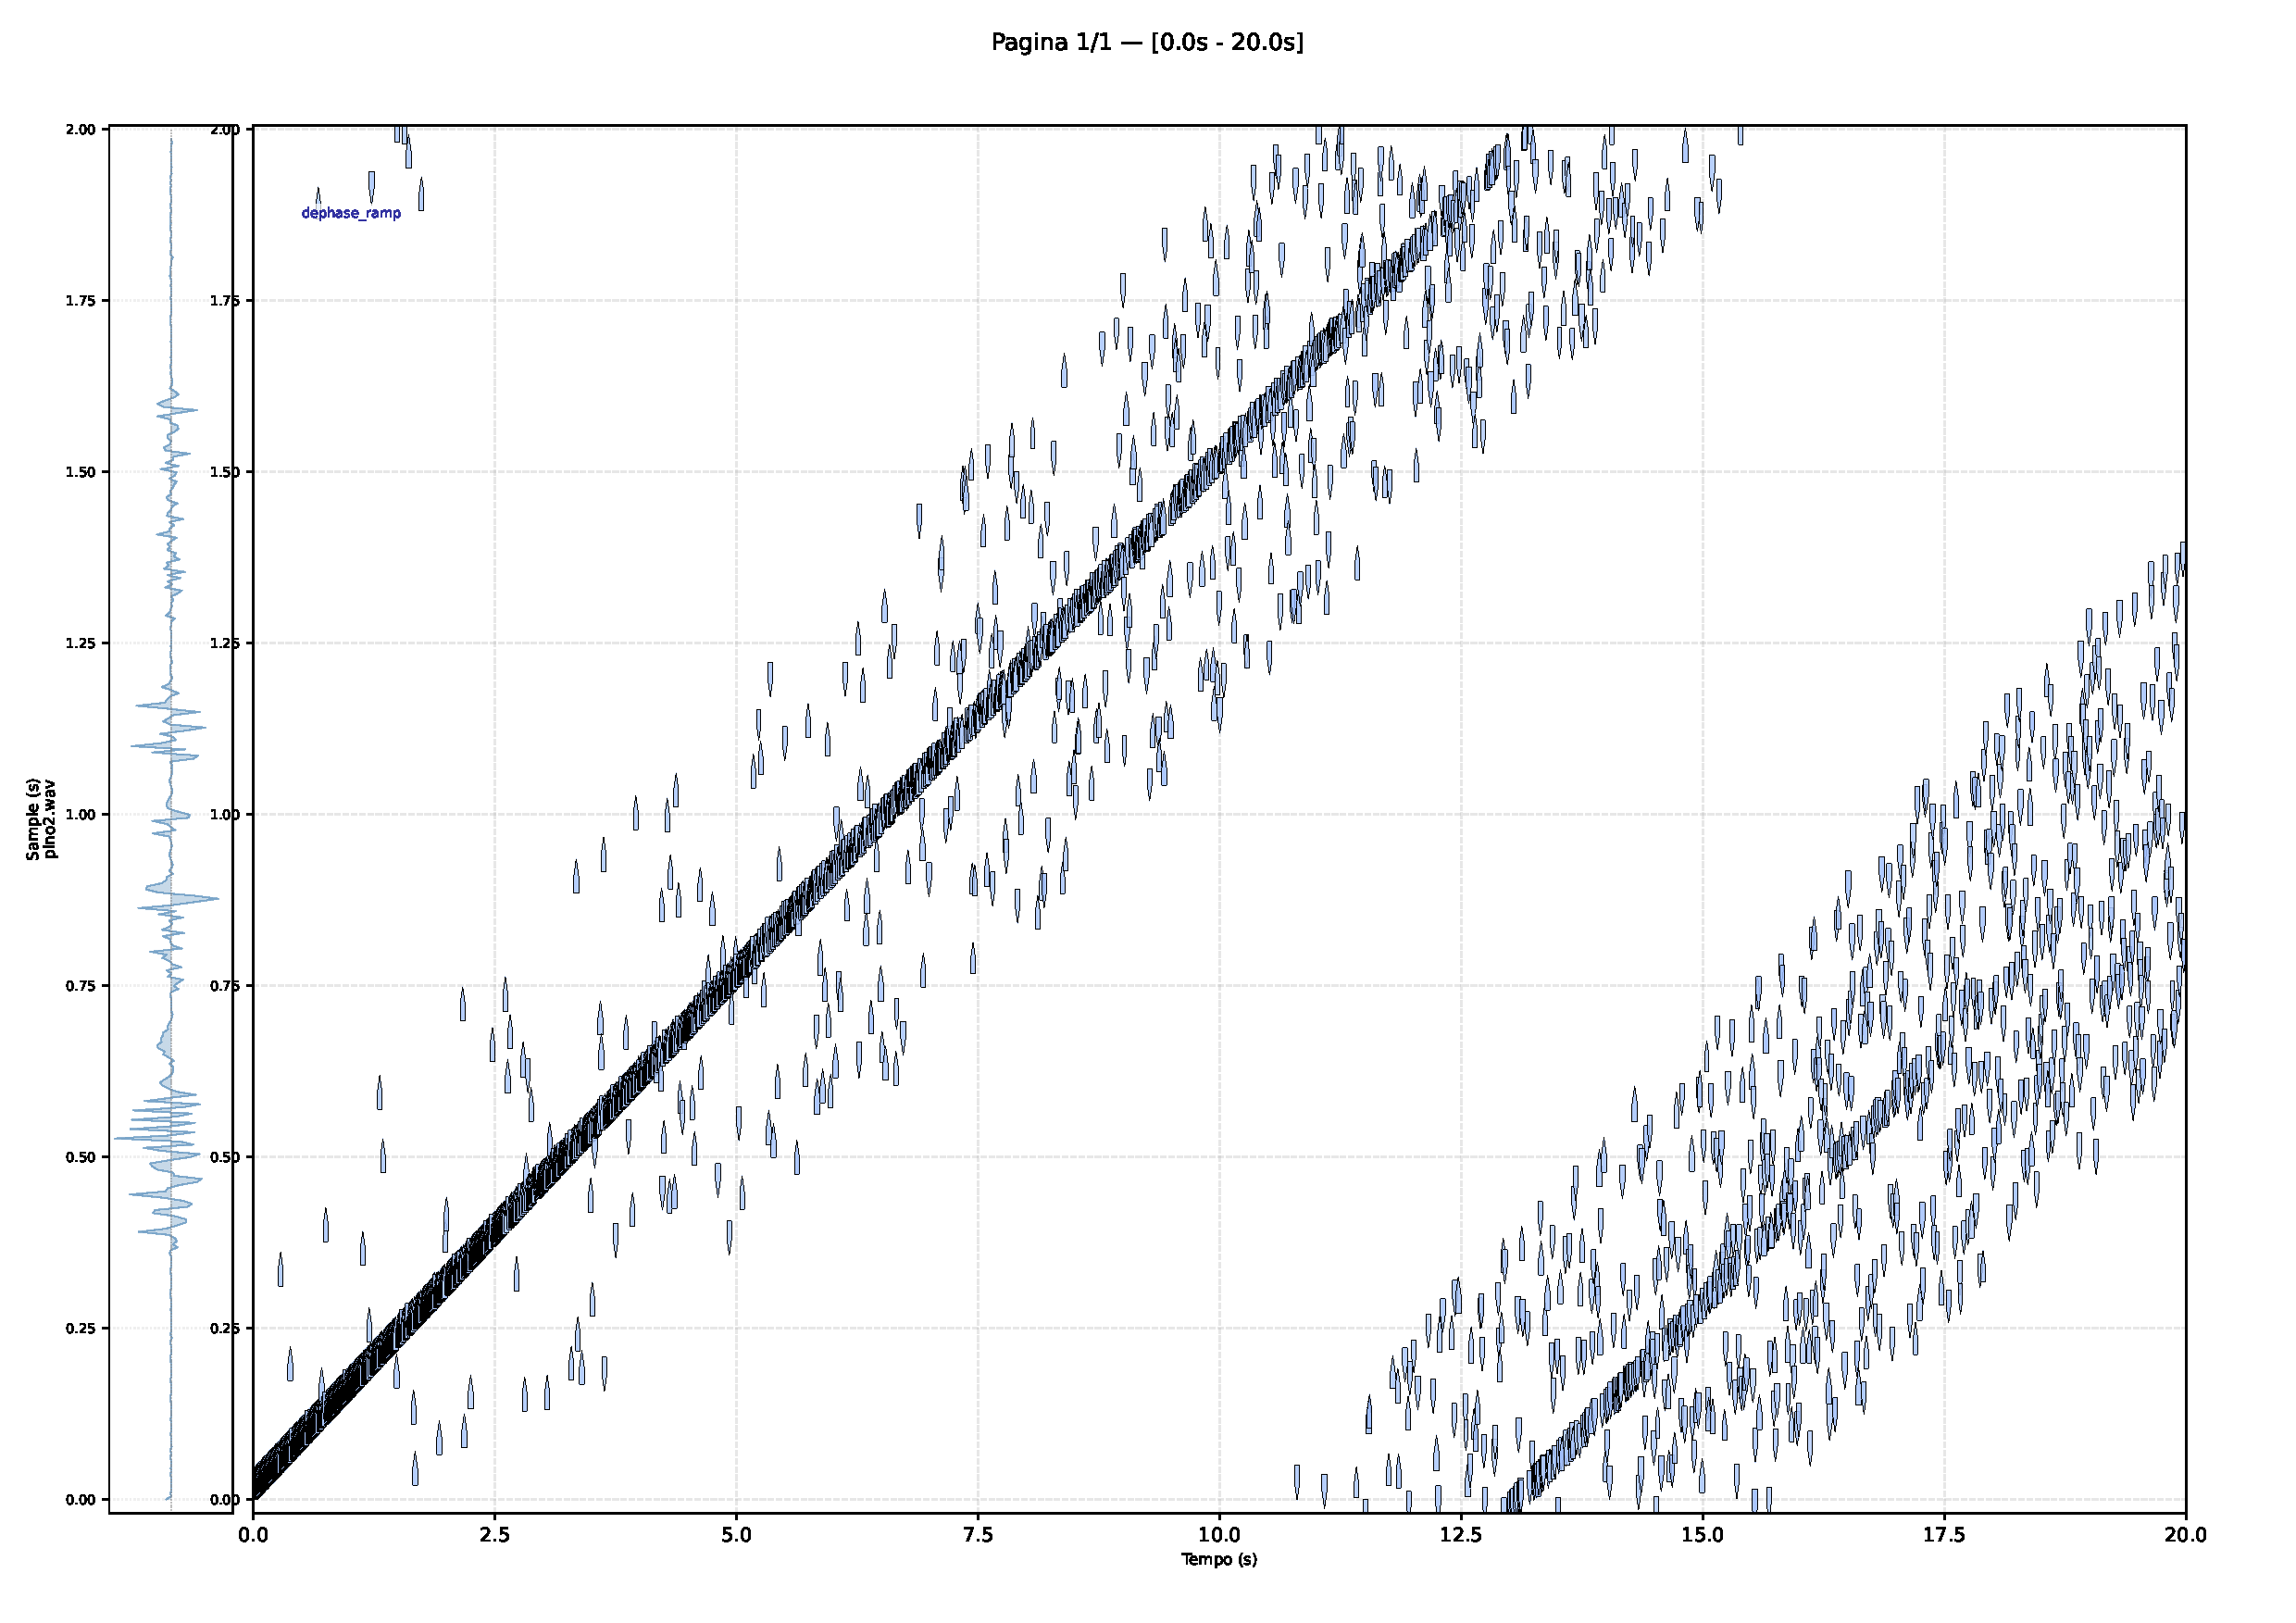
\includegraphics[width=\columnwidth]{examples/ex1_dephase/ex1_dephase_score.pdf}
  \caption{Partitura dell'esempio \texttt{ex1\_dephase} (20~s). Asse
    orizzontale: tempo; verticale: posizione di lettura nel buffer
    sorgente; colore: \texttt{pitch\_ratio} per-grano. La sola variabile
    è \texttt{dephase}, che sale da $0$ a $100$: a sinistra una banda
    netta (nessun grano dephased, lettura coerente), a destra una nuvola
    che si allarga (dispersione del pointer, pan, volume, durata e
    inversione del verso entrano in gioco con probabilità crescente). Il
    \texttt{.yml} sorgente è in
    \texttt{examples/ex1\_dephase/}.}
  \label{fig:score}
\end{figure}

% ================================================================
\section{Posizionamento nella tradizione granulare}\label{sec:tradizione}

Il paradigma granulare si fonda sulla proposta di Gabor~\cite{Gabor1947}
di rappresentare il suono come matrice di quanti elementari sul piano
tempo-frequenza, soggetti al principio di indeterminazione
$\Delta t \cdot \Delta f \geq 1$. La sua implementazione computer
introduce il problema di controllo già richiamato; Roads~\cite{Roads1978}
lo affronta col pattern \emph{front-end~$\to$~engine} e, nel primo
paper CIM dedicato~\cite{Roads1985cim}, formalizza il problema
d$\cdot$n (densità per durata) come motivazione del DSL, il
\emph{frame} come unità sopra il grano e il \emph{polygon} come
notazione: tre precursori diretti dei costrutti di
\S\ref{sec:architettura}.

Truax~\cite{Truax1988} consolida la pratica granulare in tempo reale
sul DMX-1000 e ne fissa il vocabolario. Il suo ricorso al
non-determinismo statistico va letto con precisione: si tratta di
\emph{economia di mezzi}.
Specificare individualmente migliaia di grani al secondo è
impraticabile: gli \emph{«score files [\dots] are usually so large
that they are impractical to handle»} (p.~14). L'approccio statistico
(la tendency mask) risponde a questa intrattabilità. Egli progetta anche la
macro-struttura armonica: in \emph{Riverrun} \emph{«the superimposition
of many similar and spectrally related subevents produces a clearly
defined and controllable macro-level texture»}, mentre \emph{«the
presence of any particular frequency component at the micro-level
[\dots] can only be statistically determined»} (pp.~24--25). La tendency
mask è esplicitamente \emph{«a continuum between deterministic and
stochastic choices»} (p.~23): macro progettato e micro statistico
coesistono. Il contributo compositivo del paradigma è questa discesa
\emph{nell'intimo del segnale}, che impone un orientamento
macroscopico di altro tipo e che Truax~\cite{Truax1994} formalizza
come separazione micro/macro: la granulazione \emph{«links frequency
and time at the micro level [so it] makes it possible to treat these
two variables independently at the macro level»} (p.~44). Il sistema
qui descritto eredita la tendency mask come modello di controllo
(\S\ref{sec:architettura}), senza ereditarne la postura sul tempo
reale.

Il contesto italiano sviluppa una linea offline autonoma. De~Poli e
Piccialli~\cite{DePoliPiccialli1988} elaborano una granulazione
additiva pitch-synchronous con grani come risposte FIR e controllo
formantico: il pattern \emph{precompute-once~/~reuse-many} della
finestra prototipo è precursore CIM del generatore di finestre del
sistema. Di~Scipio~\cite{DiScipio1991cim}, oltre a esplicitare il
vincolo hardware del tempo differito (\emph{«queste procedure sono
attualmente implementate in tempo differito, su un IBM PC~286
[\dots] un problema [\dots] sta nella quantità di RAM»}), sceglie
come controllo le mappe caotiche deterministiche ($x_{n+1}=f(x_n)$),
una famiglia distinta dalla tendency mask statistica, qui non
ripresa. Arcella e Silvestri~\cite{Arcella2012}, ricostruendo
\emph{Analogique~B}, fissano in ambito CIM la topologia
\emph{algoritmo~$\to$~score~$\to$~Csound~$\to$~audio}
\emph{«factor[ed] [\dots] in two»} (p.~147): è il precursore più
vicino della pipeline (anche se relativo a un brano di letteratura). Il sistema se ne distingue per il livello di
astrazione del modulo di specifica (YAML dichiarativo + IR Python),
che non emette direttamente score Csound.

Sul piano del regime temporale, il sistema si colloca all'estremo di
un arco documentato in ambito CIM: dal tempo differito per necessità
hardware (Roads, Di~Scipio) alla sua rottura real-time, di cui
Lippe~\cite{Lippe1993cim} segna sul piano CIM il punto di transizione
introducendo la distinzione fra \emph{granular synthesis} e
\emph{granular sampling} a cui questo lavoro appartiene, fino al
ritorno volontario al differito. 
In Di~Scipio l'offline è presentato come un vincolo
di macchina; qui è una scelta. La tendency mask, che Truax usava per
necessità in tempo reale, è ripresa in differito: il costo di tenere
ogni parametro sotto gli occhi se lo carica il differito stesso.

Sul versante real-time contemporaneo, EmissionControl2~\cite{Roads2021}
affianca alla granulazione uno \emph{Scan Display}: forma d'onda con
scanner sovrapposto in tempo reale, la rappresentazione viva del «dove
sto leggendo» mentre il suono scorre. La partitura qui descritta
condivide l'oggetto, la posizione di lettura, ma ne ribalta il
regime temporale. Dove lo \emph{Scan Display} è un cursore che segue
l'esecuzione, la partitura è una mappa statica dell'intera popolazione
di grani, ispezionabile fuori dal tempo dell'esecuzione.

% ================================================================
\section{Implicazioni teorico-compositive}\label{sec:implicazioni}

%Le scelte architetturali descritte hanno implicazioni compositive. Quando il controllo scende nell'intimo del segnale, il rapporto fra una specifica parametrica e il suo esito percettivo è difficile da prevedere a tavolino, e va verificato generando e riascoltando.

%Questa necessità di osservazione iterativa, prima che l'esito sia prevedibile, è ciò che Di~Scipio~\cite{DiScipio1994} descrive nei \emph{models of detailed sonic design}: la forma del suono è \emph{«more operationalized than produced»}, esito di un ciclo di osservazione del comportamento micro-strutturale, e non immagine sonora preesistente. È la partitura grafica a chiudere questo riscontro, e a renderlo ispezionabile parametro per parametro.

Il ritorno al tempo differito, in un momento in cui il tempo reale è
disponibile, non è regressione. Le prime implementazioni adottavano
l'offline per vincolo hardware~\cite{Roads1978,DiScipio1991cim}; il
sistema qui descritto lo adotta per scelta. La posizione è enunciata,
quasi trent'anni prima dell'implementazione su laptop, da
Risset~\cite{Risset1999}: \emph{«Composition is not --- or should not be
--- a real-time process. [\dots] Non real-time operation is necessary to
free oneself of the arrow of time and its tyranny, of the dictates of
haste, instancy, habits, reflexes. Writing music implies prediction and
elaboration»} (p.~37). Risset elenca cinque drawback strutturali del real-time (complessità
sonora limitata, flessibilità ridotta rispetto al software synthesis,
impossibilità del \emph{bookkeeping} compositivo, effimerità
tecnologica, la musica su supporto come tradizione viva), e con essi
fonda la legittimità del differito senza ricorso alla nostalgia. Due
hanno risposta tecnica diretta nel sistema: l'avere ogni parametro
sotto gli occhi nel DSL e la possibilità di ispezionarlo nella
partitura grafica rispondono al mancato \emph{bookkeeping}, dove \emph{«the significance
of the control settings is often unknown or obscure»} (p.~34); la
separazione fra specifica testuale e renderer pluggable risponde
all'effimerità e mantiene il brano leggibile e ri-renderizzabile
oltre la vita del singolo motore audio.

Gli strumenti, infine, non sono neutri. La forma del DSL orienta le decisioni
compositive che rendono possibili: \emph{«tools and technologies used to
produce a musical work are not neutral but incorporate knowledge that
influence the choices of the composer»}~\cite{Arcella2012}. La postura
qui descritta è personale e situata: una configurazione operativa di
cui il sistema è insieme strumento e argomento.

% ================================================================
\section{Conclusioni e sviluppi}

Il sistema descritto realizza una postura compositiva attorno al tempo
differito: un DSL YAML come linguaggio di intenzioni parametriche
validato in scrittura, una partitura grafica con asse verticale sulla
posizione di lettura come retroazione diagnostica, un workflow STEMS con
cache incrementale ed export DAW che mantiene praticabile il loop lungo.
L'architettura disaccoppiata (renderer NumPy nativo dietro
un'interfaccia estensibile) è additiva per costruzione: nuovi
back-end e nuove modalità di output non toccano il nucleo. Tre
direzioni restano aperte al futuro: un editor grafico che astragga
ulteriormente la specifica al di sopra del codice; un percorso
real-time opzionale per i contesti che lo richiedono; l'uso didattico
del sistema come ambiente in cui la tecnica granulare si studia
attraverso la composizione. La postura compositiva che questo modo di
lavorare rende possibile, e il ciclo di riscrittura che la sostiene,
meritano una trattazione a sé, oggetto di un lavoro dedicato.

% ----------------------------------------------------------------
\bibliographystyle{plain}
\bibliography{refs}

\end{document}
